\chapter{Il livello di rete: data plane}
\section{Considerazioni sul livello di rete}
A differenza dei livelli precedenti il livello di rete si trova anche nei router e negli elementi nel network core. Il ruolo primario del data plane nel 
livello di rete di ogni router\`e quello di permettere il forwarding dei datagrammi dai suoi input links verso gli output links, il ruolo primario del 
control plane \`e di coordinare queste operazioni di forwarding per router in modo che il datagramma arrivi a destinazione. 
\subsection{Forwarding e routing: il data e control plane}
Il roulo primario del livello di rete \`e quello di muovere dati dal mittente al destinatario. Affinch\`e questo avvenga vegono individuate due funzioni
fondamentali:
\begin{itemize}
\item Forwarding: quando un pacchetto arriva ad un router input link deve essere spostato nell'appropriato output link. Tale pacchetto pu\`o essere anche 
bloccato o copiato e mandato a multipli destinatari.
\item Routing: il livello di rete deve saper determinare la route o il cammino preso dal pacchetto mentre si sposta dal mittente al destinatario. 
L'algoritmo che implementa questa funzionalit\`a \`e detto algoritmo di routing.
\end{itemize}
Un elemento chiave in ogni router \`e la sua tabella di forwarding: un router forwards un pacchetto controllando i valori di alcuni campi nell'header e 
usando questi valori per indicizzare la tabella. Il valore salvato per quei campi indica il link di output dove deve essere mandato il pacchetto. 
\subsubsection{Approccio tradizionale al control plane}
Le tabelle di forwarding sono determinate da un algoritmo di routing che viene eseguito su ogni router e pertanto entrambe le funzioni di forwarding e di
routing sono contenute in esso. La funzione dell'algoritmo di routing di un router comunica con altre attraverso per computare i valori della tabella di 
forwarding. Questa comunicazione avviene attraverso un protocollo di routing. 
\subsubsection{Approccio SDN al control plane}
In questo approccio le tabelle di routing sono computate e distribuite da un controller separato fisicamente dai router e il router possiede solo la 
funzione di forwarding. La comunicazione tra questi elementi avviene attraverso lo scambio di messaggi contenenti le tabelle di routing e altre componenti. 
Questo approccio \`e al centro del software-defined networking (SDN) in quanto il controller \`e implementato in software. 
\subsection{Network service model}
Il network service model determina le caratteristiche dei servizi offerti dal livello di rete. Possono essere:
\begin{multicols}{2}
\begin{itemize}
\item Consegna garantita.
\item Consegna garantita con ritardo limitato.
\item Consegna di pacchetti in ordine.
\item Sicurezza.
\end{itemize}
\end{multicols}
Il livello di rete garantisce un solo servizio: il servizio di best-effort. In questo servizio n\`e la consegna n\`e l'ordine sono garantiti.
\section{Componenti di un router}
\begin{figure}[h]
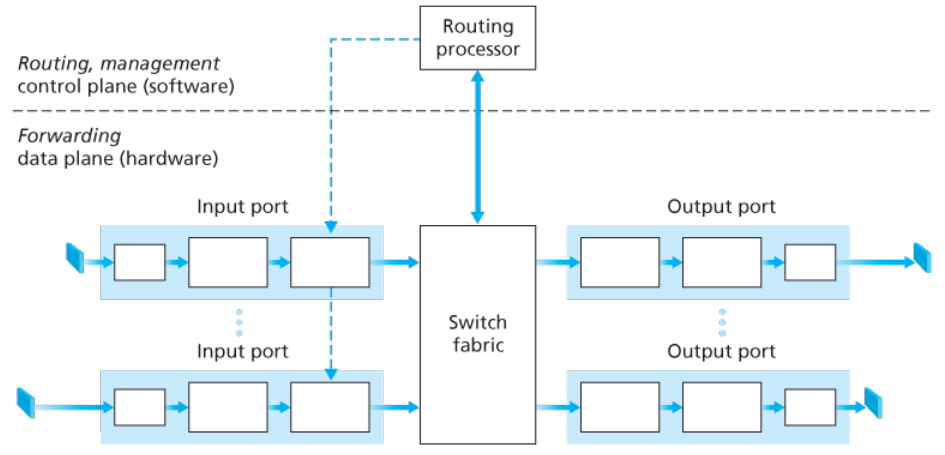
\includegraphics[width=\textwidth]{Router.png}
\caption{Architettura di un router}
\end{figure}
\begin{itemize}
\item Porte di input: una porta di input svolge la funzione di livello fisico di interrompere un link fisico entrante nel router, funzioni di livello di 
link necessarie per interoperare con il livello di link all'altro capo del link. Inoltre viene anche svolta una funzione di lookup dove viene consultata la 
tabella di forwarding per determinare a quale porta di output verr\`a forwarded il pacchetto attraverso la switching fabric. I pacchetti di controllo sono
forwarded da una porta di input al processore del router.
\item Switching fabric: questa componente connette le porte di input con le porte di output e costituisce essa stessa una rete. 
\item Porte di output: questa componenente salva i pacchetti ricevuti dalla switching fabric e li trasmette al link facendo le necessarie operazioni 
di livello di link e fisico. Quando il link \`e bidirezionale la porta corrispondente di input viene accoppiata a quella di output. 
\item Processore di routing: svolge funzioni di control plane: nei router tradizionali esegue il protocollo di routing , mantiene le tabelle di routing e 
relative informazioni di link state e computa la tabella di forwarding. Nei router SDN \`e responsabile per la comunicazione con il controller. Svolge oltre
funzioni di gestione della rete.
\end{itemize}
A causa della necessit\`a di operare a velocit\`a elevatissime tutte queste componenti sono implementate in hardware.
\subsection{Processi alle porte di input e forwarding basato sulla destinazione}
Le funzioni di line termination e di livello di link processing della porta di input implementano il livello di link e fisico per quel link di input. Il 
lookup svolto nella porta di input \`e centrale per le funzioni del router: qui viene utilizzata la tabella di forwarding per detrminare la porta di input
al quale il pacchetto dovr\`a essere inviato attraverso la switching fabric. La tabella di forwarding \`e computata dal processore di routing o ricevuta dal
controller. La tabella di routing \`e copiata dal processore alla porta di input attraverso un bus diverso in modo da evitare un bottleneck causato dalla
chiamata di un processo centrale. Si consideri ora il caso in cui la porta di output \`e determinata unicamente dall'indirizzo di destinazione: a causa
del gran numero di indirizzi possibili non \`e possibile utilizzare un algoritmo brute-force. Per migliorare le prestazioni si utilizza una regola di 
longest prefix matching: il router ritorna dalla tabella l'indirizzo tale per cui attraverso il lookup si \`e trovato il pi\`u lungo prefisso 
corrispondente. Vengono inoltre utilizzate tecniche pi\`u efficienti di una ricerca lineare come la memorizzazione delle tabelle in DRAM con SRAM come
cache o ternary content addressable memory (TCAM). Una volta che la destinazione del pacchetto \`e stata determinata entra nella switching fabric. In alcuni
casi un pacchetto potrebbe essere temporaneamente bloccato se pacchetti da altre porte la stanno utilizzando, venendo posto in una coda e programmato per
entrare nella switching fabric in un secondo momento. Oltre al lookup devono comunque essere svolte altre operazioni: processamento al livello fisico e di
link, i campi di numero di versione, checksum e time-to-live devono essere controllati e gli ultimi due riscritti e i contatori per la gestione di rete 
devono essere aggiornati.
\subsection{Switching}
Lo switching pu\`o essere ottenuto in vari modi:
\begin{itemize}
\item Switching attraverso la memoria: nei primi router, normali computer una porta di input notificava il processore di routing attraverso un interrupt 
dell'arrivo di un pacchetto che veniva copiato dalla porta nella memoria del processore che estraeva l'header, svolgeva l'operazione di lookup e lo copiava
nel buffer della porta di output. 
\item Switching attraverso un bus: in questo approccio la porta di input trasferisce il pacchetto direttamente verso la porta di output lungo un bus 
condiviso. Tutte le porte di output ricevono il pacchetto ma solo quella appropriata lo mantiene. Solo un pacchetto alla volta pu\`o trovarsi nel bus.
\item Switching attravreso una rete di interconnessione: si utilizza un crossbar switch che consiste di $2N$ bus che connettono $N$ porte di input ad 
altrettante porte di output. Ogni bus verticale si interseca con uno orizzontale ad un crosspoint che pu\`o essere aperto o chiuso. Un pacchetto da A a Y
trover\`a chiuso il crosspoint nell'intersezione dei bus di A e Y. Questo switch si dice non bloccante in quanto un pacchetto pu\`o attraversarlo a patto 
che non abbia lo stesso output di un altro.
\end{itemize}
\subsection{Processing delle porte di output}
Le porte di output prendono i pacchetti nei corrispettivi buffer, li selezionano, li rimuovono dal buffer, svolgono le funzioni di livello di link e fisico
e inviano il pacchetto al link.
\subsection{Queuing}
Le code di pacchetti possono accadere nei buffer delle porte di input o in quelli delle porte di output. La dimensione di queste code dipende dalla 
quantit\`a di traffico, dalla velocit\`a della switching fabric e dalla velocit\`a della linea. \`E quando queste code vengono riempite fino al massimo che
vengono persi dei pacchetti. Si supponga che le linee di input e output abbiano tutte la stessa velocit\`a $R_{line}$ e che ce ne sono $N$ per tipo. Si 
assuma che tutti i pacchetti abbiano una lunghezza fissa e arrivino alle porte in maniera sincrona. Si definisca $R_{switch}$ il tasso di trasmissione della
switching fabric. Se questo \`e uguale a $NR_{line}$ nessuna coda verr\`a creata alle porte di input. 
\subsubsection{Input queuing}
In caso che $R_{switch}$ sia minore di $NR_{line}$ pu\`o succedere che pacchetti debbano essere messi in coda nell'attesa che vengano inviati alle porte di
input. Si supponga una crossbar switching fabric con velocit\`a di link identiche e che un pacchetto possa essere trasferito ad una porta di output nello
stesso tempo in cui viene ricevuto dal link di input e i pacchetti sono mossi verso l'output in modo FCFS (first-come first-served), pacchetti multipli 
possono essere trasferiti simultaneamente a patto che abbiano output diversi. Pu\`o nascere un evento di head-of-the-line blocking (HOL) in quanto un 
pacchetto incodato deve aspettare per il trasferimento perch\`e quello prima di lui \`e bloccato da un altro. A causa di questo evento la coda potrebbe 
crescere illimitatamente e pertanto causare perdita di dati.
\subsubsection{Output queuing}
Si supponga $R_{switch}$ uguale  $NR_{line}$ e che gli $N$ pacchetti che arrivano da ognuna delle porte di input debbano essere inviati nella stessa porta 
di output. In questo caso durante la trasmissione di un pacchetto arrivano alla porta $N$ nuovi pacchetti e questi dovranno essere incodati. Eventualmente
questa coda si potrebbe riempire causando perdita di pacchetti. Quando non c'\`e pi\`u abbastanza memoria per salvare un pacchetto si deve scegliere se 
droppare il pacchetto appena arrivato (drop-tail) o uno in coda. Un'altra azione potrebbe essere quella di marcare un pacchetto prima che questo si 
verifichi in modo da inforamare dell'esistenza di congestione. Un numero di regole di packet dropping e marking \`e conosciuto come active queue management
(AQM). Uno dei pi\`u diffusi \`e il random early detection (RED). Una conseguenza di questo incodamento \`e che un packet scheduler alla porta di output 
deve decidere quale pacchetto trasmettere. Le dimensioni della coda variano e vengono scelte in base  a $RTT\cdot C\text{(link capacity)}$ o $\frac{RTI\cdot 
C}{N}$, dove $N$ il numero di TCP flows.
\subsection{Packet scheduling}
\subsubsection{First-in First-out (FIFO)}
Un pacchetto viene incodato se il link \`e occupato e quando il buffer \`e pieno entrano in gioco le discard policies. La politica FIFO invia pacchetti 
nello stesso ordine con cui arrivano alla porta di output. 
\subsubsection{Priority queuing}
In questa politica i pacchetti che arrivano al link sono separati in classi di priorit\`a . Ogni classe di priorit\`a ha tipicamente la sua coda. Quando 
deve scegliere che pacchetto trasmettere viene scelto dalla coda non vuota con la priorit\`a pi\`u alta. All'interno di ogni coda vige una politica FIFO.
\subsubsection{Round robin e weighted fair queuing (WFQ)}
Come nel priority queuing i pacchetti sono divisi in classi e un round robin scheduler alterna i servizi tra le classi. Una disciplina di work-conserving 
queuing non permetter\`a al link di rimanere idle fino a che ci sono pacchetti da trasmettere controllando immediatamente la classe successiva se quella
che considera \`e vuota. Una forma generalizzata di round robin \`e il weighted fair queuing, una disciplina work-conserving che si muove tra le classi
ciclicamente secondo un peso $w_i$ ed \`e garantita una frazione di servizio pari a $\frac{w_i}{\sum w_j}$ dove il denominatore \`e la somma dei pesi delle
classi con pacchetti. Ogni classe ottiene un throughput di almento $R\frac{w_i}{\sum w_j}$.
\section{Il protocollo di internet: IPv4, indirizzamento, IPv6}
\subsection{Formato del datagramma IPv4}
\begin{figure}[h]
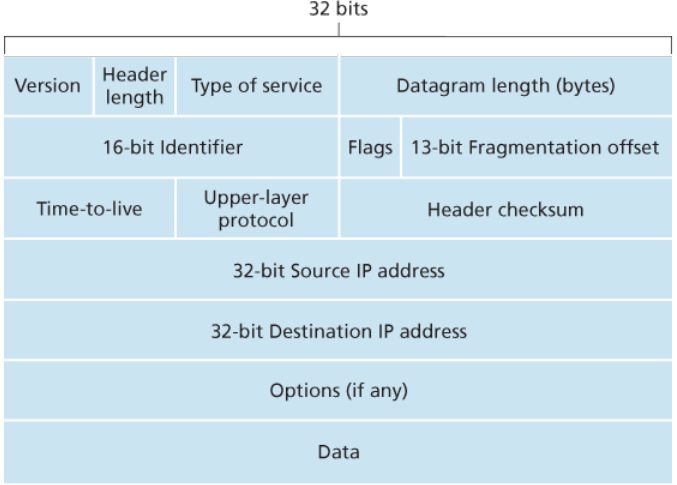
\includegraphics[width=\textwidth]{IPv4Datagram.png}
\caption{formato del datagramma IPv4}
\end{figure}
I campi nel datagramma IPv4 sono:
\begin{itemize}
\item Version number: questi 4 bit specificano la versione di IP utilizzata in modo che il router possa interpretare gli altri bit dell'header.
\item Header length: essendo che un header del datagramma pu\`o contenere informazioni di lunghezza variabile si deve notificare dove inizia il payload.
La lunghezza tipica \`e di 20 bytes.
\item Type of service: utilizzati per determinare degli utilizzi del datagramma come ECN o servizi real-time.
\item Datagram length: la lunghezza totale del datagramma misurata in bytes, \`e a 16 bit.
\item Identificatori, flags, segmentation offset.
\item Time-to-live: utilizzato per impedire che datagrammi circolino infinitamente. Questo campo \`e decrementato di $1$ ogni volta che un datagramma 
attraversa un router. Quando raggiunge zero deve essere droppato.
\item Protocol: tipicamente utilizzato quando il datagramma raggiunge la destinazione indica il tipo di protocollo di transport layer utilizzato. 6 per TCP
e 17 per UDP.
\item Header checksum: aiuta a individuare errori di bit in un ricevuto datagramma IP. Computato considerando 2 bytes nell'header come numeri e sommandoli 
tra di loro in complemento a 1. A causa del TLL viene ricomputato in ogni router. 
\item Source e destination IP addresses.
\item Options: opzionali causano differenze di processing per pacchetti diversi e segmenti di lunghezza diversa.
\item Data o payload: contiene il segmento del livello di trasporto. 
\end{itemize}
\subsection{IPv4 frammentazione del datagramma}
La massima quantit\`a di dati che un link pu\`o trasportare \`e detta maximum transmission unit (MTU) e determina un limite rigido per la dimensione massima
dei datagrammi. Essendo che da mittente e destinatario possono sussistere link con MTU diverse nascono dei problemi. Quando si deve inviare un datagramma
troppo grosso in un link con MTU troppo piccolo questo viene frammentato in due frame di livello di link pi\`u piccoli. Questi frammenti devono essere 
ricomposti prima di essere inviati al livello di trasporto. La deframmentazione avviene negli end-systems. Pertanto quando un host destinatario riceve dei
datagrammi deve determinare se questi sono frammenti di un datagramma originale. Deve anche determinare quando ha ricevuto l'ultimo frammento e come i 
frammenti debbano essere riuniti. Per far questo vengono utilizzate i campi di identification, flags e segmentation offset. Quando un datagramma \`e creato
il mittente lo marca con un identificatore  aumentato per ogni datagramma inviato. Quando tale datagramma viene frammentato ogni frammento possiede lo 
stesso identificatore. L'ultimo frammento ha un flag settato a 0 in modo da essere sicuri di aver ricevuto tutti i frammenti, il fragmentation offset \`e
utilizzato per ordinare e determinare se un frammento \`e mancante. 
\subsection{Indirizzamento IPv4}
Un host possiede tipicamente un unico link verso la rete e quando IP deve mandare un datagramma lo fa lungo quel link. Il limite tra l'host e il link fisico
viene chiamato interfaccia. Un router d'altra parte \`e connesso a numerosi link e pertanto possiede altrettante inferfacce. IP richiede che ogni 
interfaccia abbia il proprio indirizzo IP. Ogni indirizzo IP consiste di 32 bits scritti tipicamente nella dotted-decimal-notation, in cui ogni byte \`e 
scritto come decimale e separato dagli altri da un punto. Ogni interfaccia in ogni host e router deve possedere un IP univoco. Una porzione dell'indirizzo
viene scelta in base alla sottorete di appartenenza dell'interfaccia. Una rete che connette delle interfacce host con un interfaccia router \`e detta
sottorete (o rete IP). L'indirizzamento IP assegna un indirizzo alla sottorete $xxx.xxx.xxx.xxx/24$ dove $/24$ indica che i 24 bit pi\`u a sinistra detti
subnet mask definiscono l'indirizzo della sottorete e ogni host addizionale aggiunto alla sottorete avr\`a quei 24 bit uguali. Per determinare le subnets
si stacchi ogni interfaccia dal suo router o host creando delle reti isolate che vengono dette subnet. L'assegnazione di indirizzi IP dell'internet \`e
detta classless interdomain router (CIDR) che generalizza la cognizione di indirizzamento per le subnets. L'indirizzo IP a 32 bit \`e diviso in due 
parti e viene indicato con $a.b.c.d/x$ dove $x$ indica il numero di bit per la prima parte. Gli $x$ bit pi\`u significativi formano il prefisso o prefisso
di rete dell'indirizzo. Ad un'organizzazione vengono tipicamente assegnati IP contigui con lo stesso prefisso e sono gli unici bit considerati dai router
all'esterno dell'organizzazione. I rimanenti $32-x$ bits vengono utilizzati per fare forwarding sui pacchetti all'interno dell'organizzazione. Viene 
riservato l'indirizzo IP di broadcast 255.255.255.255 in cui il pacchetto viene duplicato in tutti gli host nella stessa sottorete. 
\subsubsection{Ottenere un blocco di indirizzi}
In ordine per ottenere un blocco di indirizzi IP per un'organizzazione si deve contattare un ISP che mette a disposizione indirizzi da un numero di 
indirizzi a sua disposizione ancora pi\`u grande. Lo fa aumentando la dimensione della subnet mask. L'interezza degli indirizzi IP \`e gestita dalla 
Internet corporationfor assigned names and numbers (ICANN) che si occupa di allocare gli indirizzi IP e di gestire i server DNS di root, assegna nomi di 
dominio e risolve dispute riguardo essi. Alloca indirizzi verso regristri locali che formano l'Address support organization dell'ICANN (ASO-ICANN) che 
gestiscono l'allocazione e la gestione di indirizzi all'interno della loro regione. 
\subsubsection{Ottenere un indirizzo IP per l'host: il Dynamic host configuration protocol}
Una volta che un'organizzazione ha ottenuto un blocco di indirizzi li pu\`o assegnare ad ogni interfaccia al suo interno. Gli indirizzi IP dei router sono
tipicamente configurati manualmente, mentre quelli degli host sono configurati attraverso il dinamic host configuration protocolo (DHCP) che permette ad un
host di ricevere un indirizzo IP automaticamente. L'host pu\`o ricevere lo stesso indirizzo IP ogni volta che si connette alla rete o ottenerne uno
temporaneo alla connessione. DHCP mette inoltre a disposizione all'host informazioni sul primo router (default gateway), la subnet mask e l'indirizzo del
server DNS locale. Questo protocollo \`e detto plug-and-play e zeroconf. DHCP \`e un protocollo client-server. Un client \`e tipicamente un nuovo host che
vuole ottenere informazioni per la configurazione di rete e un indirizzo IP per s\`e. Nel caso pi\`u semplice ogni subnet possiede un server DHCP. Se non 
\`e presente un DHCP relay agent che conosce la posizione del server DHCP per la rete \`e necessario. Per un nuovo host il protocollo DHCP \`e composto da
quattro fasi: 
\begin{itemize}
\item DHCP server discovery: il primo compito dell'host \`e quello di trovare il server DHCP ed \`e fatto attravreso un DHCP discover message che un client
invia attraverso un pacchetto UDP alla porta 67 con la broadcast definition dell'indirizzo IP e un questo host con indirizzo IP 0.0.0.0 l'host lo incapsula
in in frame di livello di link e fa un broadcast a tutti i nodi presenti nella sottorete.
\item DHCP server offer: il server che riceve il DHCP discovery message risponde al client con un DHCP offer message inviato attraverso il broadcast IP. 
Questo messaggio contiene il transacion ID del discover message, l'indirizzo IP proposto e l'IP lease time solitamente settato a ore o giorni. 
\item DHCP request: il client sceglie tra i server offer arrivatigli e risponde con un DHCP request message che fa echoing sui parametri di configurazione.
\item DHCP ACK: il server risponde al request message attraverso un DHCP ACK message che conferma i parametri richiesti. 
\end{itemize}
Una volta completati questi messaggi il client pu\`o utilizzare l'indirizzo IP consegnatogli. Se vuole continuare a utilizzarlo dopo la fine del lease time
DHCP mette a disposizione dei meccanismi per rinnovare l'indirizzo. Non si possono mantenere connessioni TCP se si sposta tra le sottoreti. 
\subsection{Network address translation (NAT)}
Il network addres translation viene utilizzato per facilitare la gestione di piccoli uffici o istallazioni casalinghe (SOHO) oltre a permettere di 
connettere pi\`u dispositivi all'internet. Un NAT-enabled router ha un'interfaccia parte della rete di casa. Tutte le interfacce in questa rete hanno la 
stessa subnet mask e lo spazio di indirizzo $/8$ \`e uno dei tre riservato per una rete privata o una realt\`a con reti private. Il NAT enable router non
sembra un router alla rete esterna ma viene considerato come come un singolo dispositivo con un singolo indirizzo IP, ovvero nasconde i dettagli della rete
casalinga al mondo esterno. Tutti questi indirizzi vengono ottenuti attraverso DHCP (dal server dell'ISP per il router e da quello del router per i 
dispositivi interni). Essendo che tutti i datagrammi che arrivano al router NAT hanno lo stesso indirizzo, per ottenere il destinatario corretto viene 
utilizzata una tabella di traduzione NAT e vengono inclusi i numeri di porta oltre agli indirizzi IP.
\subsection{IPv6}
I maggiori cambi nel formato del datagramma sono:
\begin{itemize}
\item Expanded addressing capabilities: la dimensione dell'inirizzo IP \`e aumentata da 32 a 128 bit. 
\item Un header di 40 byte fissi eliminando le opzioni in modo da permettere un router processing pi\`u veloce.
\item Flow labeling: in modo da marcare pacchetti per cui il mittente richiede una gestione speciale. 
\end{itemize}
\begin{figure}[h]
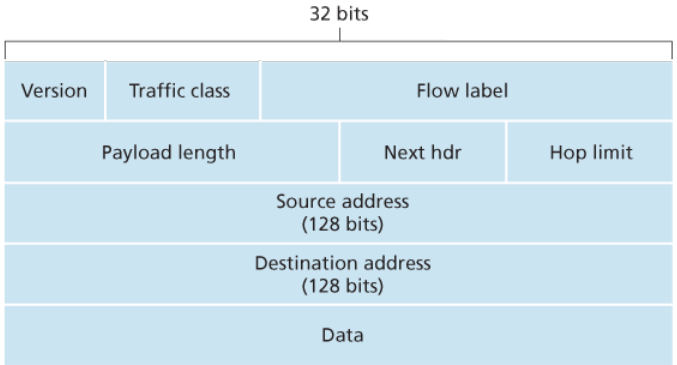
\includegraphics[width=\textwidth]{IPv6Datagram.png}
\caption{formato del datagramma IPv6}
\end{figure}
I seguenti campi sono definiti in IPv6:
\begin{itemize}
\item Version: il campo di 4 bit che indica la versione di IP utilizzata (con valore 6 per IPv6).
\item Traffic class: un campo a 8 bit come il TOS in IPv4.
\item Flow label: un campo a 20 bit che identifica datagrammi appartenenti ad un flow.
\item Lunghezza del payload: un unsigned integer che determina la lunghezza del payload del datagramma. 
\item Next header: identifica il protocollo del segmento contenuto.
\item Hop limit: questo valore \`e diminuito ogni volta che il datagramma attraversa un router e quando raggiunge zero il pacchetto viene eliminato.
\item Source and destination addresses: a 128 bit ognuno.
\item Data payload.
\end{itemize}
IPv6 a differenza di IPv4 non mette a disposizione un servizio di frammentazione: se un pacchetto \`e troppo grande lo droppa e invia al mittente un 
messaggio di ICMP che notifica che il pacchetto era troppo grande. Header checksum in quanto altri livelli lo compiono gi\`a e considerato ridondante. 
\subsubsection{Transizionare da IPv4 a IPv6}
Per effettuare la transizione da IPv4 a IPv6 viene utilizzato l'approccio del tunneling: quando un datagramma IPv6 trova un router ad IPv4 viene 
impacchettato in un nuovo datagramma IPv4 il nodo alla fine del tunneil IPv4 capisce che contiene un datagramma IPv6, lo estrae e lo forward. 
\section{Forwarding generalizzato e SDN}
Nel forwarding generalizzato una tabella match-plus-action generalizza la tabella di forwarding incontrata precedentemente. Questi dispositivi vengono 
riferiti come packet switch. La tabella in ogni packet switch \`e computata da un controller esterno. Ogni input in una tabella di match-plus-action 
chiamata flow table include:
\begin{itemize}
\item Un insieme di campi header ai quali un pacchetto in entrata sar\`a matchato utilizzando memoria TCAM, se non c'\`e nessun match il pacchetto pu\`o 
essere droppato o inviato al controller per ulteriore processing. 
\item Un insieme di contatori sono aggiornati mano a mano che i pacchetti sono matchati.
\item Un insieme di azioni da essere intraprese quando si trova un match. 
\end{itemize}
\subsection{Matching}
\begin{figure}[h]
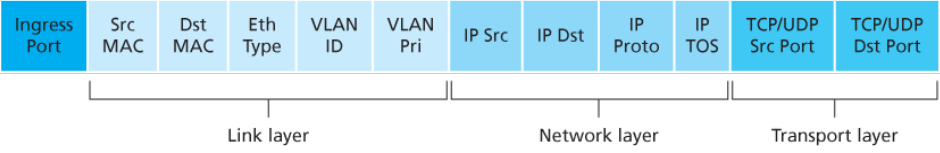
\includegraphics[width=\textwidth]{FlowTableEntry.png}
\caption{formato del datagramma IPv6}
\end{figure}
Si noti come l'astrazione fatta sul pacchetto perfette di accedere a dati provenienti da diversi livelli dello stack di rete. Le entries possono avere 
wildcards negli indirizzi IP e hanno una priorit\`a associata. 
\subsection{Action}
Dopo che avviene un match esiste una lista di zero o pi\`u azioni di processing da effettuare per quanto riguarda il pacchetto. Alcune delle pi\`u 
importanti sono:
\begin{itemize}
\item Forwarding: un pacchetto potrebbe essere inviato su una, alcune o tutte le porte di output o inviato al controller.
\item Dropping: il pacchetto viene droppato se non ci sono entries.
\item Modify-field: un campo del pacchetto viene modificato.
\end{itemize}